\documentclass{article}
\usepackage{CJKutf8}
\usepackage{graphicx}
\usepackage{math_blog}

\title{布朗运动与随机过程的构造}
\author{Anqiao Ouyang}
\date{July 29, 2025}

\newcommand{\Title}{布朗运动与随机过程的构造}
\newcommand{\Column}{Stochastic Differential Equations I}
\newcommand{\Author}{Anqiao Ouyang}

\begin{document}
\begin{CJK*}{UTF8}{gbsn}

\maketitle

\section{引言}

在对现实世界中的不确定性进行建模时，传统的常微分方程（ODE）往往显得力不从心。我们需要能够处理随机性的数学工具，便引出了随机微分方程（SDE）。作为本系列的第一篇文章，我们将从数学角度系统地介绍这一基础层面。我们将定义什么是随机过程，解释什么是滤过与适应性，并以布朗运动为核心案例展开深入讨论，然后理解布朗运动作为 SDE 驱动项的严谨逻辑，并学习其构造方式。

读者应具备一定的数学基础，主要包括高中微积分，基础概率论（特别是对概率空间、随机变量、分布与独立性等概念的掌握），初步的测度论直觉。尽管本文将尽量通过直观解释引导理解，但若希望深入掌握其背后的逻辑结构，仍建议读者在阅读过程中适时回顾或补充相关基础知识。

\textit{Ouyang又在挖系列坑了...希望会继续写下去吧XD}

\section{随机过程的基本定义}

\subsection{形式定义}

\begin{definition}[随机过程]
设 $(\Omega, \mathcal{F}, \mathbb{P})$ 是一个概率空间，$T$ 是时间索引集（如 $T = \mathbb{N}$ 或 $T = [0, \infty)$），状态空间为 $\mathbb{R}^d$。如果对每个 $t \in T$，$X_t : \Omega \to \mathbb{R}^d$ 是 $\mathcal{F}$-可测的随机变量，则称 $\{X_t\}_{t \in T}$ 是一个取值于 $\mathbb{R}^d$ 的随机过程。
\end{definition}

从直观上看，随机过程就是一组随时间变化的随机变量。与单一随机变量不同，它的意义更像是随机性随时间扩展与积累，即关注过程本身。每一个 $\omega \in \Omega$ 对应一条样本路径 $t \mapsto X_t(\omega)$，描述了在某一具体情形下，系统的完整演化轨迹。举个例子，在金融市场中，股价可以被视为一个连续时间的实值随机过程。

定义直觉上很好理解吧？！话虽如此，要将理论进一步发展光有脑瓜子里的直觉是不够的，我们还要理解一些经典的随机过程并理解它们的结构与性质。

\subsection{泊松过程}

简单回顾一下，泊松分布常用于描述在固定时间区间内发生的稀疏、独立事件的数量，其中 $\lambda$ 表示该时间区间内事件发生的平均次数。例如，在一分钟内平均接到 3 个电话，那么该分钟内接到 $k$ 个电话的概率就服从参数为 $\lambda = 3$ 的泊松分布。

\begin{definition}[泊松分布]
设 $\lambda > 0$ 为给定的参数，称离散随机变量 $N$ 服从参数为 $\lambda$ 的泊松分布，记作 $N \sim \text{Poisson}(\lambda)$，如果其概率质量函数为：
\[
\mathbb{P}(N = k) = \frac{\lambda^k e^{-\lambda}}{k!}, \quad \forall k \in \mathbb{N}_0.
\]
\end{definition}

我们将泊松分布的概念扩展到连续时间的框架，使对象在每个时间区间的增量服从相应参数的泊松分布，即为泊松过程。

泊松过程是用于建模一系列离散事件在时间中随机发生的经典模型。事件之间彼此独立，且单位时间内事件发生的平均频率是已知的常数。这意味着我们虽然知道事件大致多久发生一次（例如每小时平均有 $\lambda$ 次事件），但却无法预测每一次事件的确切时刻。這像一种“无记忆性”，一件事情的发生是否并不会影响下一个事件出现是否的概率。

\begin{definition}[泊松过程]
一个随机过程 $\{N_t\}_{t \geq 0}$ 称为参数为 $\lambda > 0$ 的泊松过程，若满足：
\begin{itemize}
    \item 初始值为零：$N_0 = 0$ 几乎处处
    \item 增量独立性（Independent Increments）：对于任意满足 $0 \leq t_0 < t_1 < \cdots < t_n$ 的时间点，增量
    \[
    N_{t_1} - N_{t_0},\quad N_{t_2} - N_{t_1},\quad \dots,\quad N_{t_n} - N_{t_{n-1}}
    \]
    是相互独立的随机变量；
    \item 增量分布稳定性（Stationary Increments）：对任意 $s < t$，增量 $N_t - N_s$ 服从参数为 $\lambda(t - s)$ 的泊松分布，即
    \[
    \mathbb{P}(N_t - N_s = k) = \frac{[\lambda(t - s)]^k}{k!} e^{-\lambda(t - s)}, \quad \forall k \in \mathbb{N}_0
    \]
    \item 样本路径性质：对几乎所有 $\omega \in \Omega$，映射 $t \mapsto N_t(\omega)$ 是右连续并具有左极限（即 càdlàg），且仅在可数个时刻发生单位跳跃，即$\Delta N_t := N_t - N_{t-} \in \{0, 1\}, \quad \text{and} \quad \{t :\Delta N_t = 1\}$ 在每个有限区间内是有限集合。
\end{itemize}
\end{definition}

换言之，它描述的是在单位时间内事件的累计次数这一随机变量的行为。当我们将这个思想推广到“任意时间区间”时，就得到了一条随时间演化的事件计数路径，也就是泊松过程。实际上，泊松过程的定义正是建立在“任意时间长度的事件计数，始终服从参数与时间长度成比例的泊松分布”的假设之上。

\subsection{布朗运动（Wiener 过程）}

布朗运动是连续时间、连续状态空间的基本随机过程。与泊松过程那种阶梯式、分段常数的跳跃路径不同，布朗运动展现出的是连续扰动与非平稳走势的典型特征，这也正是它在 SDE 中被用作驱动项（噪声源）的原因。

\paragraph{高斯分布回顾}

我们回顾一下，一个实值随机变量 $X$ 被称为服从参数为 $\mu \in \mathbb{R}$ 和 $\sigma^2 > 0$ 的正态分布（或高斯分布），记作 $X \sim \mathcal{N}(\mu, \sigma^2)$，如果其概率密度函数为：
\[
f(x) = \frac{1}{\sqrt{2\pi \sigma^2}} \exp\left( -\frac{(x - \mu)^2}{2\sigma^2} \right), \quad x \in \mathbb{R}.
\]

其中，$\mu$ 表示该分布的均值，$\sigma^2$ 表示方差，控制了样本的波动程度。当 $\mu = 0, \sigma^2 = 1$ 时，称为标准正态分布，记作 $\mathcal{N}(0, 1)$。正态分布是概率论中最重要的分布之一，具有对称性、单峰性和稳定性等性质。

\begin{definition}[布朗运动]
设 $(\Omega, \mathcal{F}, \mathbb{P})$ 为概率空间，$\{\mathcal{F}_t\}_{t \geq 0}$ 为满足通常条件（right-continuous, complete）的滤过。一个一维随机过程 $\{W_t\}_{t \geq 0}$ 称为标准布朗运动，若满足：

\begin{itemize}
    \item 初始值为零：$W_0 = 0$ 几乎处处；
    
    \item 独立增量（independent increments）：对于任意 $0 \leq t_0 < t_1 < \cdots < t_n$，增量
    \[
    W_{t_1} - W_{t_0},\quad W_{t_2} - W_{t_1},\quad \dots,\quad W_{t_n} - W_{t_{n-1}}
    \]
    相互独立；
    
    \item 正态增量（Gaussian increments）：对于任意 $s < t$，增量 $W_t - W_s$ 服从正态分布，满足
    \[
    W_t - W_s \sim \mathcal{N}(0, t - s)
    \]
    
    \item 样本路径连续：几乎处处，映射 $t \mapsto W_t(\omega)$ 在 $t$ 上连续。
\end{itemize}
\end{definition}

布朗运动的路径几乎处处是连续但不可导的。意味着虽然看起来平滑，其实际都是微小震荡，任何两个瞬间之间都存在不可预测的波动。直观上它像是在不断“抖动”的曲线，没有明确的方向导数。

\begin{figure}[h]
    \centering
    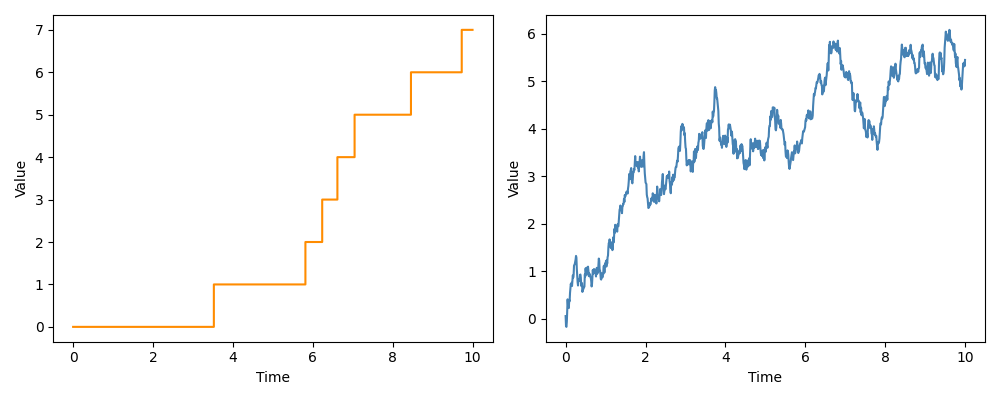
\includegraphics[width=1.0\textwidth]{./figures/1.png}
    \caption{左：泊松过程；右：布朗运动。}
    \label{fig:poisson_brownian}
\end{figure}

\section{Filtration与适应性}

\subsection{滤过的定义}

\begin{definition}[滤过]
设 $(\Omega, \mathcal{F}, \mathbb{P})$ 是一个概率空间。若 $\{\mathcal{F}_t\}_{t \geq 0}$ 是一族 $\sigma$-代数，满足
\[
\mathcal{F}_s \subseteq \mathcal{F}_t \subseteq \mathcal{F}, \quad \forall s \leq t
\]
则称 $\{\mathcal{F}_t\}$ 为一个滤过（filtration）。
\end{definition}

滤过描述了信息如何随时间逐步累积的过程。直观地说，$\mathcal{F}_t$ 表示“在时间 $t$ 之前能够观测到的所有随机事件”的集合，随着时间的推移，所能获取的信息越来越多。。

在实际分析中，我们通常要求滤过满足“常规条件”（usual conditions），即：

- 右连续性：$\mathcal{F}_t = \bigcap_{s > t} \mathcal{F}_s$；
- 完备性：$\mathcal{F}_0$ 包含所有 $\mathbb{P}$-零测集。

\subsection{适应性}

\begin{definition}[适应性]
设 $\{X_t\}_{t \geq 0}$ 是一个随机过程，若对所有 $t \geq 0$，随机变量 $X_t$ 都是 $\mathcal{F}_t$-可测的，则称该过程对滤过 $\{\mathcal{F}_t\}$ 是适应的（adapted）。
\end{definition}

适应性意味着在时间 $t$ 时，过程 $X_t$ 的取值是“可以被知道的”，即 $X_t$ 不依赖未来的信息。我们通常只允许“非预知性”的过程作为被积函数或系数函数，故这个条件在随机积分与SDE中至关重要。

我们只能对已经发生的过程信息进行积分，不能对未来“偷看”（所以做错了选择就不要抱着赌徒心理想着“下次不会了”哦:），在伊藤积分的定义中，这样的适应性是一个基本要求，我们将在下一章详细讨论。

\subsection{自然滤过与预测性}

自然滤过是研究随机过程时最常用的滤过之一。在大多数情况下，我们默认某一过程的行为仅依赖于它自身的历史，因此自然滤过成为刻画信息流动的基本结构。

\begin{definition}[自然滤过]
设 $\{X_t\}_{t \geq 0}$ 是一个随机过程，其自然滤过（natural filtration）定义为：
\[
\mathcal{F}^X_t := \sigma(X_s : 0 \leq s \leq t)
\]
即由该过程在区间 $[0, t]$ 内的所有取值所生成的最小 $\sigma$-代数。整个族 $\{\mathcal{F}^X_t\}_{t \geq 0}$ 构成一个随时间增长的信息结构，描述了“该过程自身在每个时刻之前可观测的信息”。
\end{definition}

例如，布朗运动 $W_t$ 对其自然滤过
\[
\mathcal{F}^W_t := \sigma(W_s : 0 \leq s \leq t)
\]
是适应的，因为 $W_t$ 的值完全由历史路径决定。

预测性过程比适应过程更严格，它要求每个时刻的值都“可以在严格更早的时间预测到”。这类过程在后续定义随机积分时非常重要，它确保被积函数不会依赖未来的信息。在大多数应用中，左连续的适应过程都是预测性的。尽管本章不涉及积分，但理解预测性的基本形式，有助于在后续伊藤积分构造中掌握积分对 integrand 的可测性要求。

\begin{definition}[预测性过程]
设 $\{\mathcal{F}_t\}_{t \geq 0}$ 是一个滤过。一个过程 $\{H_t\}_{t \geq 0}$ 被称为是该滤过下的预测性过程（predictable process），如果它在 $[0,\infty) \times \Omega$ 上是对预测 $\sigma$-代数 $\mathcal{P}$ 可测的，其中 $\mathcal{P}$ 是由以下类过程生成的最小 $\sigma$-代数：
\begin{itemize}
    \item 对每个 $t$ 左连续的适应过程；
    \item 分段常数过程，其在区间 $(t_i, t_{i+1}]$ 上取 $\mathcal{F}_{t_i}$-可测的常值。
\end{itemize}
\end{definition}

值得注意的是，适应过程已经不允许“预知未来”，但预测性过程更严格，它甚至不允许你在“当下”做出决定，只能基于严格的“过去”行动。如果你在每个时刻 $t$ 观察了窗外天气（也就是用了当前时刻的信息 $\mathcal{F}_{t}$ 之后再决定是否带伞，那你的策略 $H_t$ 是 $\mathcal{F}_t$-可测的，属于适应性过程。要做到预测性过程的话，你必须在 $t$ 时刻到达之前，已经根据过去的天气情况（即 $\mathcal{F}_{t-}$）决定是否带伞。

这听起来有点怪，那凭什么它还叫“预测”？在这里“预测”体现在的是人可以提前知道它将怎么做的事实，而非直觉上的“预测未来”，好一个迷惑！

\section{布朗运动的构造}

布朗运动作为随机微分方程中的核心驱动项，其理论基础建立在一套清晰的概率结构之上。为了确保这类过程在概率空间中确实存在，并可以被模拟、分析和应用，我们需要从多个角度系统性地构造布朗运动。

\subsection{布朗运动的公理定义}

在 Definition~2.4 中，我们已经给出了标准布朗运动的公理化定义，它由四个基本性质构成：初始为零、具有独立增量、增量服从正态分布，以及样本路径几乎处处连续。這種“连续却不可预测”的随机扰动模型的路径是连续的，却没有导数；增量服从高斯分布，但彼此之间独立，且服从平稳的时间结构。

这里我们对布朗运动的公理化定义的四个主要条件做一個简单的回顾並理解其数学意义：

\begin{itemize}

    \item \textbf{初始值为零}：$W_0 = 0$

    这一条件确保布朗运动从一个确定的起点开始，使过程在时间上具有一致性。在数值模拟、建模或理论分析中，明确的初始条件用于统一各种布朗路径的比较与归一化。

    \item \textbf{独立增量}：不同时间区间的增量相互独立

    对任意时间点序列 $0 \leq t_0 < t_1 < \cdots < t_n$，增量 $W_{t_1} - W_{t_0}, W_{t_2} - W_{t_1}, \dots$ 是相互独立的。这个条件意味着布朗运动在每个时间段内的变化不受过去影响，体现出过程的“无记忆性”。

    \item \textbf{正态增量}：增量服从正态分布，对任意 $s < t$，增量 $W_t - W_s \sim \mathcal{N}(0, t - s)$。这说明布朗运动在任意时间区间上的扰动大小（方差）与区间长度成正比，且其分布是高斯分布，体现过程的“均匀波动性”。

    \item \textbf{样本路径连续}：几乎处处连续的样本路径

    对于几乎所有 $\omega \in \Omega$，映射 $t \mapsto W_t(\omega)$ 是连续函数。虽然路径连续，但布朗运动几乎处处不可导，因此轨迹极为不规则。这种结构是布朗运动可以建模“持续但无方向”的随机扰动的原因。

\end{itemize}

\subsubsection{样本路径的连续性与不可导性}

布朗运动的样本路径是连续的，但却几乎处处不可导。具体来说，尽管布朗运动的轨迹没有跳跃，具有平滑的外观，但它在每一点处都不可微分。这一特性是它区别于许多其他随机过程的特点。

\paragraph{路径连续性}
布朗运动的路径连续性意味着，过程的每一个样本路径随着时间的推移不会突然中断或跳跃。在数理上，布朗运动在任何有限时间区间内，几乎所有的样本路径都是右连续的，且没有跳跃点。这一点与泊松过程等“跳跃过程”形成鲜明对比。

\paragraph{不可导性}
尽管布朗运动的路径是连续的，但它的路径在几乎每个时间点都没有定义导数，即布朗运动几乎处处不可导。这种不可导性反映了布朗运动的高度不规则性，数学上也表现为其路径的粗糙度。这是因为布朗运动的增量是随机的，并且随着时间的流逝，它的“微小波动”逐渐变得越来越频繁，导致其没有稳定的导数。

\subsection{协方差结构与高斯过程}

布朗运动作为一个典型的随机过程，其最重要的性质之一是它是一个**高斯过程**。这意味着，布朗运动的任意有限维分布都是多元正态分布，其协方差结构非常关键。布朗运动的协方差结构为：
\[
\mathbb{E}[W_s W_t] = \min(s, t)
\]
布朗运动在任意时间点的值不仅与当前时刻的扰动有关，还与历史信息有关。

\paragraph{高斯过程}
一个高斯过程是指它的任何有限维分布都服从多元正态分布。布朗运动是高斯过程的一个特例，因为对于任意的时间点 $t_1, t_2, \dots, t_n$，布朗运动的联合分布是多元正态分布，且其均值为零，协方差为 $\mathbb{E}[W_s W_t] = \min(s, t)$。即较早的时间点对后续时间点的变化有一定影响，而这种影响随着时间的推移逐渐减弱。它也意味着布朗运动的增量是平稳的，但仍然是随机的。

布朗运动的协方差结构是随机过程的建模的基础。此外，布朗运动的高斯性质使得它在理论上易于处理，因为高斯过程的性质（如线性组合的闭合性、条件分布等）使得它在许多分析方法中都能得到非常方便的应用。

这些性质为我们提供了布朗运动的行为特征，但它们并没有告诉我们如何确保这样的过程确实存在。也就是说尽管我们已经定义了布朗运动的属性，仍然需要证明在某些概率空间中，存在一个过程，满足这些公理化条件。

\subsubsection*{Kolmogorov存在定理}

为了证明布朗运动的存在性，我们需要使用Kolmogorov存在定理，从一组已知的有限维分布中构造一个满足这些分布的随机过程。如果一组有限维分布满足一致性条件（即，在不同时间点的联合分布满足预期的分布规律），那么可以构造一个随机过程，使得它的有限维分布与这些一致。

\begin{theorem}[Kolmogorov存在定理]
设 $\{F_t\}_{t \geq 0}$ 为一族满足一致性条件的有限维分布族，即对任意时间 $0 \leq s < t$，其联合分布满足：
\[
\mathbb{P}(X_s \leq x_1, X_t \leq x_2) = \mathbb{P}(X_s \leq x_1) \cdot \mathbb{P}(X_t \leq x_2 | X_s = x_1)
\]
那么，存在一个概率空间 $(\Omega, \mathcal{F}, \mathbb{P})$ 和一族随机变量 $\{X_t\}_{t \geq 0}$，使得它们的有限维分布与 $F_t$ 完全一致。也就是说，存在一个随机过程，使得它在每个有限维分布下满足上述条件。

\end{theorem}

在布朗运动的构造中，我们将利用 Kolmogorov存在定理来从布朗运动的有限维分布（即每个时间段内的增量分布）推导出一个随机过程。通过定义这些增量服从正态分布，并满足独立性等条件，我们能够构造出一个满足布朗运动所有公理的过程。

\subsection{Levy-Ciesielski构造}

Levy-Ciesielski 构造方法提供了一种将布朗运动从离散过程推导出来的方式。该方法通过将布朗运动的连续路径表示为一系列离散随机游动的极限，从而为布朗运动的理论和数值仿真提供了一种优雅的构造手段。

Levy-Ciesielski 构造是基于布朗运动路径的小波展开。假设我们有一组独立的标准正态随机变量 $\{Z_k\}$，这些随机变量构成了离散过程的增量。通过对这些增量的加权和，并按照特定的时间间隔进行分段，我们可以构造出布朗运动的连续路径。将布朗运动看作是一个无限多次的小步伐的极限过程，每一次小步伐都是从一个离散过程（如对称随机游动）中抽取的。这通过适当缩放和加权离散随机过程，能够生成布朗运动的路径。

设一组基于二进制小波基底的随机变量 $\{Z_k\}$，通过如下的级数展开来构造布朗运动的样本路径：
\[
W_t = \sum_{k=1}^{\infty} 2^{-\frac{k}{2}} Z_k \mathbf{1}_{[2^{-k}, 2^{-k+1})}(t)
\]
其中，$\{Z_k\}$ 是一组独立的随机变量，服从 $\mathcal{N}(0,1)$ 的标准正态分布，$\mathbf{1}_{[a,b)}(t)$ 是单位区间指示函数。

布朗运动的路径被表示为一系列增量的线性组合，每个增量的大小随着 $k$ 的增大而逐渐减小。这种方法实际上将布朗运动视为一个具有“无限精度”的离散过程，其中每个时间段内的扰动都可以看作是小步伐的累加，最终形成一个连续的轨迹。

Levy-Ciesielski 构造的一个重要特点是它能够从离散随机游动出发，生成一个平滑的连续过程，且在构造过程中能够保留布朗运动的所有基本统计性质，包括独立增量、正态分布增量和路径连续性。

虽然 Levy-Ciesielski 构造数学上非常简洁，但在实际应用中可能会因为计算复杂度而受到限制。尤其是在需要生成精确路径时，这种方法需要处理大量的小波系数，从而对计算资源提出较高要求。因此，在实际数值仿真中，常常会结合其他方法进行近似计算。

\subsection{Donsker定理}

我们不妨换一个视角来看布朗运动。通过将离散时间的对称随机游动（symmetric random walk）在极限下逼近为布朗运动。Donsker定理表明，如果我们将一个适当缩放的离散过程（如对称随机游动）推向极限，它将收敛于布朗运动。

设 $\{S_n\}_{n \geq 0}$ 是一个适当缩放的对称随机游动（例如，步长为 $1/\sqrt{n}$，每步的方向独立且均匀分布）。那么，随着 $n \to \infty$，该随机游动的路径将收敛于布朗运动 $W_t$，即：
\[
\lim_{n \to \infty} \frac{S_{\lfloor nt \rfloor}}{\sqrt{n}} = W_t
\]
这里$S_n$ 表示离散时间下的随机游动，$\lfloor nt \rfloor$ 表示在 $t$ 时刻的索引。Donsker定理实际上给出了离散过程向布朗运动转化的收敛性和极限分布。

值得注意的是其收敛性是收敛性，当时间间隔无限小，步长无限多时，离散过程的轨迹会趋向于一个连续的路径，且其增量服从正态分布。

Donsker定理不仅仅是布朗运动的理论基础，它在数值模拟、随机过程的近似计算等实际应用中具有重要意义。通过 Donsker定理，我们可以利用离散随机游动来模拟布朗运动，并通过增加时间步长的精度来近似布朗运动的轨迹。它为模拟过程提供了逼近方法，并且与 Levy-Ciesielski 构造一起，在随机微分方程的数值解法中有广泛应用。

\end{CJK*}
\end{document}
